
This section examines the hypothesis that relative socioeconomic
status \textit{within} education bins has changed for blacks relative
to whites during the study period. This kind of change could bias our
estimates of mortality change, because we assume that the latent
education ranks of blacks and whites \textit{within} the bottom 10\%
(and within other percentile groups) have not changed during the study
period. For example, if whites within the bottom 10\% were clustered
at the top of this percentile bin in 1992--94 and at the bottom of this
bin in 2016--18, then we would expect their measured mortality to rise
even if the underlying mortality-education-rank CEF is unchanged.  To
be concrete, suppose the mean white woman, conditional on being in the
bottom 10\% of all women, moved from the 7th percentile to the 3rd
percentile. Then comparing average mortality among white women in the
bottom 10\% could still be subject to selection bias, even in our
constant composition estimates, because the average white woman in the
bottom 10\% would be more negatively selected over time.

Note that Panel B of Figure~\ref{fig:robust} already rules this out as a
primary explanation for rising white mortality, by showing that
mortality is rising for the bottom 10\% of whites, not just for whites in
the bottom 10\% of the national education distribution. Nevertheless,
in this section we explore the possibility that the relative status of
whites in the bottom 10\% of the entire educational distribution has
shifted relative to blacks.

Because education data is interval censored (i.e. we only know that
someone is a high school dropout, but we do not observe how close they
were to completing high school), we cannot measure the education
percentile more precisely. However, we can examine whether the
socioeconomic status of white dropouts has changed relative to black
dropouts on other measures. We focus on income as measured in the
Current Population Survey.

First, we use the granular information on incomes in the CPS to rank
all people by income within each gender, age and education bin in each
year. We then compute the mean income rank for whites and blacks
within each of the four education groups used in the body of the
paper.  Figure~\ref{fig:income_ranks} plots the results of this
exercise for women and men aged 50--54. The figures show that mean
income ranks for blacks and whites, conditional on education level,
have remained stable over time. Among women, black and white dropouts
have approximately equal income rank throughout the sample
period. Among high school graduates, the relative status of whites is
increasing relative to that of blacks, which would bias us
\textit{against} finding increases in mortality. Among men, whites
have higher average income ranks within every education bin, but their
relative advantage is stable over time.  Changing relative latent
education rank \textit{within} observed education bins therefore
cannot explain any of the rise in mortality of white dropouts.
\clearpage
\begin{figure}[H]
  \caption{Average Income Ranks for 50--54 year old whites and blacks}
  \label{fig:income_ranks}
  \begin{center}
    Panel A: Women \\
      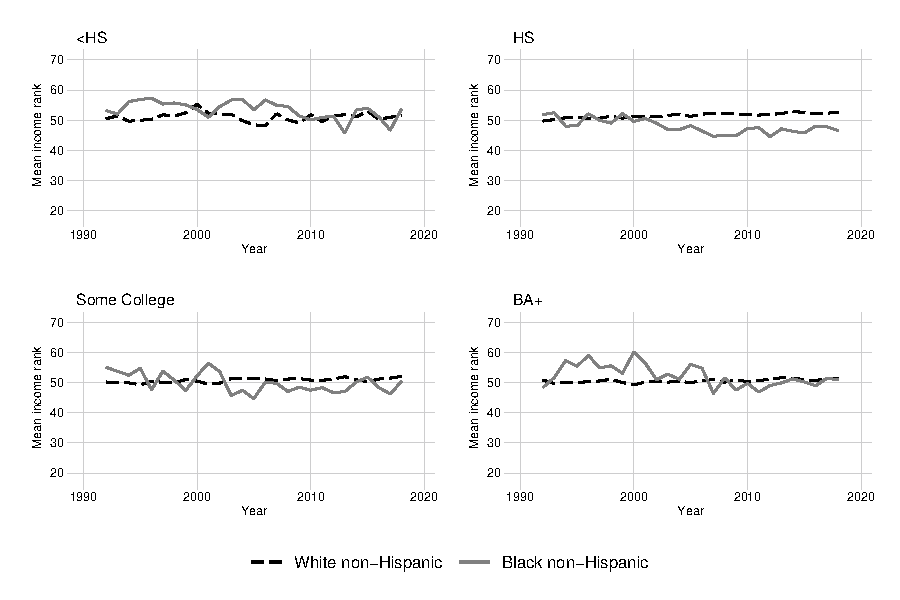
\includegraphics[scale=.75]{\mortalitypath/mean_within_rank_50_2_comb} \\
  \end{center}
  \begin{center}
    Panel B: Men \\
      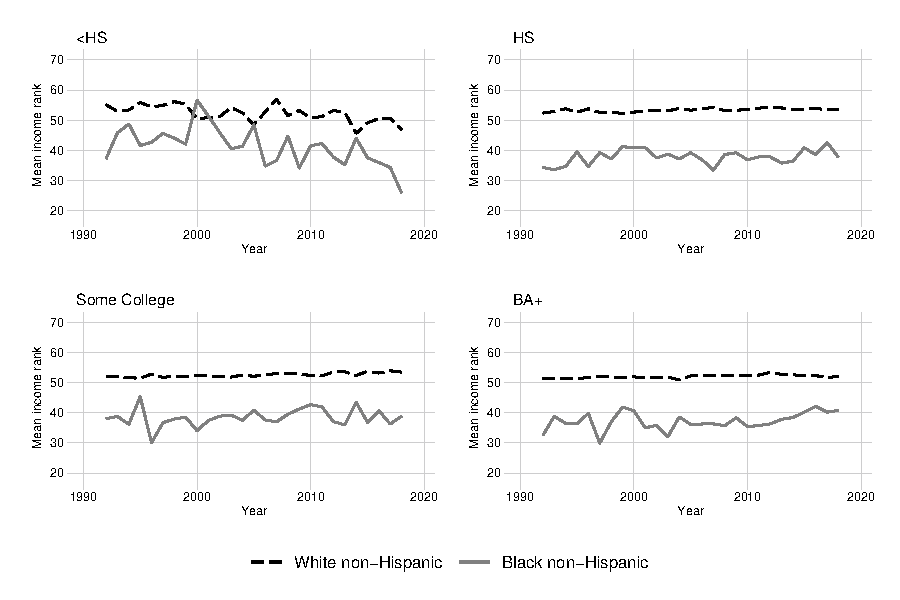
\includegraphics[scale=.75]{\mortalitypath/mean_within_rank_50_1_comb} \\
  \end{center}
\end{figure}

\scriptsize{ Note: The figure shows the average income rank within
  age, gender and education bins for non-Hispanic white and
  non-Hispanic black men and women at different education levels. Source: CPS.}
